\chapter{Detección de biomarcadores en cáncer de hígado y colon-recto}

\section{Introducción}

\section{Metodología}

\subsection{Fuente de datos}

La fuente de los datos es GDC (Genomic Data Commons) Portal, una plataforma web sobre cáncer del Instituto Nacional del Cáncer de Estados Unidos (\textit{National Cancer Institute}) \cite{GDCPortal, NationalCancerInstitute}. GDC Portal fue desarrollado por el Instituto Nacional del Cáncer de Estados Unidos, la Universidad de Chicago, el Instituto de Ontario para la Investigación del Cáncer y la empresa \textit{Leidos Biomedical Research}, y su principal fortaleza reside en la integración y armonización de diversas fuentes heterogéneas, creando así un sistema de información amplio y robusto \cite{Grossman2016}. \\

\newpage
\textbf{\textcolor{red}{Figura XX}}. Diagrama de funcionalidad y utilidad de GDC. Extraído de Grossman et al. \cite{Grossman2016}.
\begin{center}
	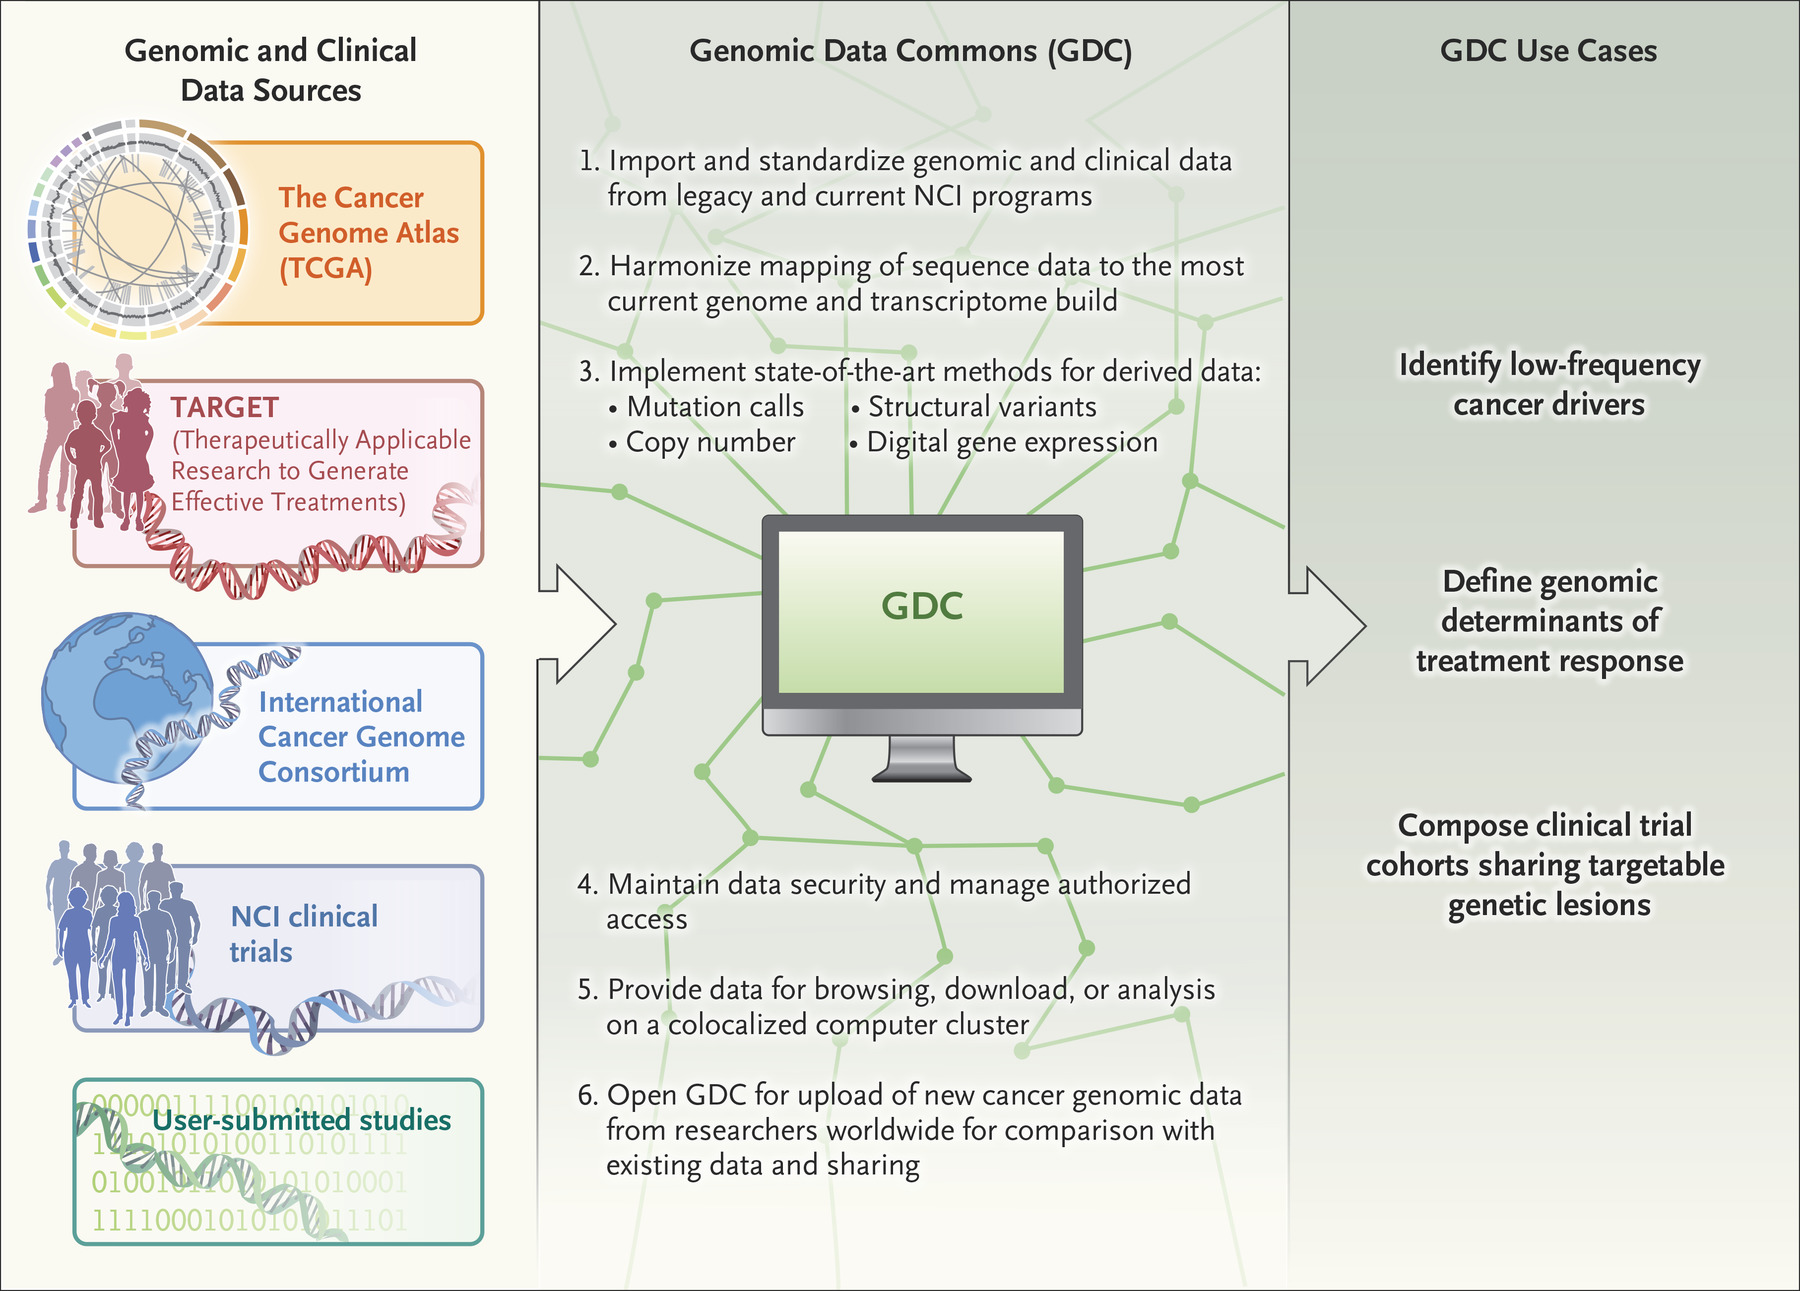
\includegraphics[width=1\textwidth]{figuras/funcionamiento_gdc.jpeg} \\
\end{center}

GDC Portal, a día 22 de Junio, contenía información sobre unos 84.000 casos, 23.000 genes y más de 3 millones de mutaciones de genes \cite{GDCPortal}. Los datos de los que dispone son muy variados, y se pueden distinguir en tres grandes categorías:

\begin{itemize}
	\item Información clínica, como la edad del sujeto, su sexo o el estadio del cáncer del que ha sido diagnosticado.
	\item Información genética y transcriptómica proveniente de diversos proyectos de investigación.
	\item Imágenes de tejidos tumorales y sanos.
\end{itemize} 

Algunos de estos datos son abiertos, mientras que para otros es necesario solicitar acceso.

\subsection{Análisis}

Para el análisis se ha utilizado el software estadístico R \cite{R} y el paquete \texttt{KnowSeq} (v.1.2.0), librería que ha sido desarrollada por los tutores del presente trabajo, y en la que el autor ha contribuido con algunas nuevas funciones y pequeñas modificaciones \cite{KnowSeq}. El paquete está además disponible en Bioconductor, una relevante plataforma de código abierto en R para el análisis de datos en genómica y transcriptómica \cite{Gentleman2004}.\\

\textcolor{red}{Otros paquetes de R con versiones y referencias! Por relevancia citar paquetes como edgeR y limma}

\section{Resultados: cáncer de hígado}

\subsection{Características clínicas de los pacientes}

\subsection{Detección de biomarcadores}

\subsubsection{Validación cruzada}

\subsubsection{Validación en test}

\section{Resultados: cáncer de colon-recto}

\subsection{Características clínicas de los pacientes}

\subsection{Detección de biomarcadores}

\subsubsection{Validación cruzada}

\subsubsection{Validación en test}

\section{Conclusiones}

\textcolor{red}{Interpretar resultados con cautela: ver pág. 65 de \cite{CastilloSecilla2020} (referencias 77-79).}\\
